\feelchapter{Heat sink}
            {Heat sink}
            {Baptiste Morin, Christophe Prud'homme}
            {cha:heatsink}

This problem considers the performance of a heat sink designed for the thermal management of high-density electronic components. The heat sink is comprised of a base/spreader which in turn supports a number of plate fins exposed to flowing air. We model the flowing air through a simple convection heat transfer coefficient. From the engineering point of view, this Problem illustrates the application of conduction analysis to an important class of cooling problems: electronic components and systems. \\ \\
Our interest is in the conduction temperature distribution at the base of the spreader. The target is to study how the heat transfer occures with different parameters on our heat sink. The heat generated by high-density electronic components is such that it's very expensive to cool large structures (data center). The cooling optimization is consequent in the run for decreasing operating costs.

\noindent A classical thermal CPU cooler looks like this 

\begin{figure}[!h]
\centering
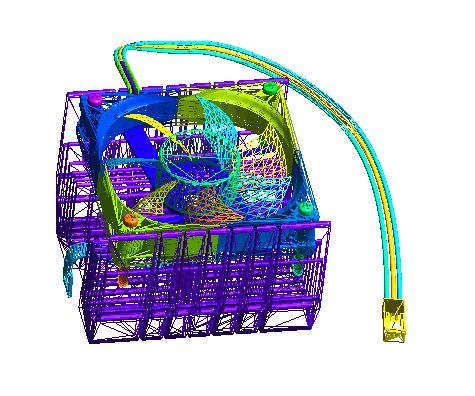
\includegraphics[width=.45\linewidth]{heatsink/complete_cooler.png}
\caption{Mesh of a classical CPU cooler}
\end{figure}

\noindent We are here going to describe how it is theorically working and how it is impleted with \feel. 

\section{Problem description}
\subsection{Domain}

We consider here a classical "radiator" which is a CPU heat sink. Those types of coolers are composed with a certain number of plate fins exposed to flowing air or exposed to a ventilator. Regarding the periodicity and geometry of our concern, we can make our study on a characteristic element of the problem : a half cell of the heat sink single thermal fin with its spreader at the basis. Let's take a look at the geometry of our problem :

\begin{figure}[!h]
\centering
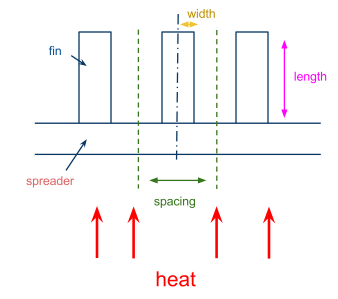
\includegraphics[width=.45\linewidth]{heatsink/sink_geom.png}
\caption{Geometry of heat sink}
\end{figure}

Our study is avaible in 2 or 3 dimensions, depending on the application's parameters. You'll see later how to work with it. Let's see on which meshes we are working on :
\begin{figure}[!h]
\begin{minipage}[b]{.50\linewidth}
\centering
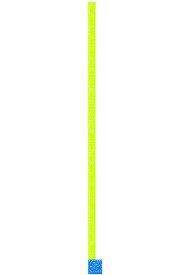
\includegraphics[width=.45\linewidth]{heatsink/mesh_2d.png}
\caption{2D mesh}
\end{minipage}
\begin{minipage}[b]{.50\linewidth}
\centering

\includegraphics[width=.45\linewidth]{heatsink/mesh_3d.png}
\caption{3D mesh}
\end{minipage}
\end{figure}

We consider the physical domain $\varOmega (\mu)$ where $\mu = (\mu_1, ...,\mu_p)$ represents the parameters of our concern. 

\subsection{Parameters}
The implementation of thoses parameters is described in the section ~\ref{heat:param}.

\subsubsection{Biot number}
The Biot number $Bi$ is a dimensionless number used in non-steady or transient states in heat transfer calculations. It gives a simple index of the ratio of the heat transfer resistances inside  and at the surface of a body. This number determines wheter or not the temperatures insdide a body will significantly vary in space while the body heats or cools over time from a thermal gradient applied to its surface. This number is defined as 
\begin{equation}
Bi = \frac{hL_c}{k_b}
\end{equation} 
where $h$ is the heat transfert coefficient, $L_c$ is the characteristic length (commonly defined as the volume of the body divided by the surface area) and $k_b$ is the thermal conductivity of the body (here the body is the thermal fin) and is expressed in $Wm^{-1}K^{-1}$. This number has to be between $0$ and $1$, this condition is included in the parameters described in ~\ref{heat:param}. This conductivity is typically one of the parameters we are insterested in to modify. This parameter corresponds to the material choosen for the heat sink. 

\subsubsection{Material}

Here the material parameter can be described with the spreader-to-fin conductivity ratio $\kappa$. This ratio is expressed as
\begin{equation*}
\displaystyle{\kappa = \frac{\tilde{\kappa}_{sp}}{\tilde{\kappa}_{fin}}}
\end{equation*}
where $\tilde{\kappa}_{sp}$ and $\tilde{\kappa}_{fin}$ are the thermal conductivities of the spreader and the fin. In that way, we make possible the construction of a heat sink with $2$ different materials. As a consequence, if you choose the same material, the ratio will be equal to $1$. \\

\noindent The material is also caracterized with its density (factor $\rho$ in the heat equation \ref{heat:eq}), here is a list of the well-known ones :
\begin{center}
\begin{tabular}{|c|c|c|}
  \hline
  Material & Thermal conductivity ($\tilde{\kappa} at 293 K$) & Density ($\rho in kg.m^{-3}$) \\
  \hline
  \hline
  Aluminium & 0.1 & 2700 \\
  \hline
  Copper & 386 & 8940 \\
  \hline
  Gold & 314 & 19320 \\
  \hline
  Silver & 406 & 10500 \\
  \hline
\end{tabular}
\end{center}

\subsubsection{Spacing}
This parameter represents the length between two plates fin. This parameter finds its place in the periodicity condition, we denote $\lambda$ this length.

\subsubsection{Thickness}
The thickness of a platefin (divided by two here because we are working on a half cell) takes part in the heat diffusion. We call $\gamma$ this parameter.

\subsubsection{Width}

This parameter is to take into account only if you are considering the 3D issue. Typically, this parameter is linked with constructor's standards. This parameter is called \lstinline!depth! in the application's implementation.


\section{Theory}
\label{therm:equations}

\subsection{Figure}
The following figure describes the parameters and the geometry we are using in the equations to solve our 2D issue :
\begin{figure}[!h]
\centering
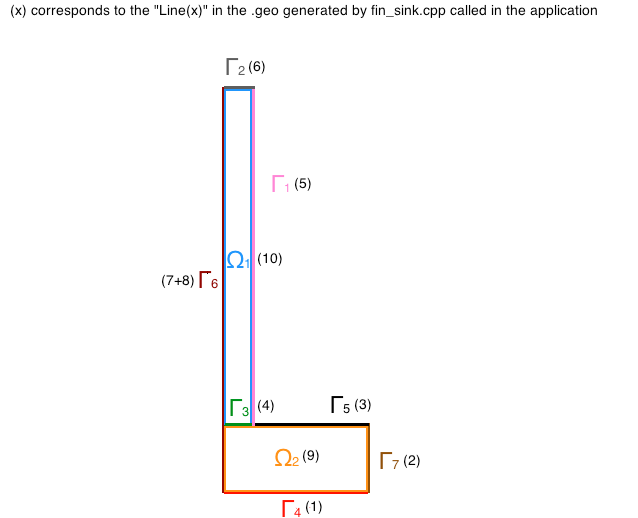
\includegraphics[width=.80\linewidth]{heatsink/figure_2d.png}
\caption{2D geometry details}
\end{figure}

The global domain is $\varOmega = \varOmega_1 \cup \varOmega_2 $ where $\varOmega_1$ is the fin's domain and $\varOmega_2$ the spreader's domain. We note $\partial\varOmega$ the border of the domain $\varOmega$. The phyical lines we are using will be noted as $\Gamma_i$ such as described above. The following figure describes the parameters and the geometry we are using in the equations to solve our 3D issue :
\begin{figure}[!h]
\centering
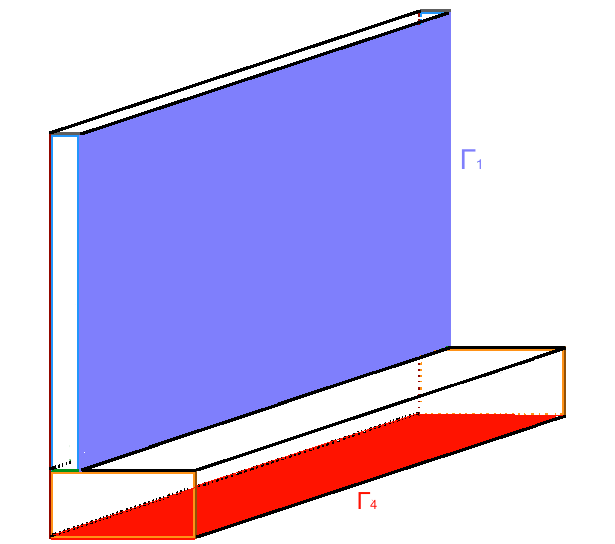
\includegraphics[width=.60\linewidth]{heatsink/figure_3d.png}
\caption{3D geometry details}
\end{figure}

\subsection{Equations}

Our concern satisfies the heat equation which reads 
\begin{equation}
\label{heat:eq}
   \begin{split}
      \kappa \Delta T - \displaystyle{\rho \frac{ \partial T}{\partial t}}  & = 0
  \end{split}
\end{equation}
\begin{equation}
\label{hom_neu}
   \begin{split}
      \displaystyle{ \kappa \frac{\partial T}{\partial n}} & =  0 \quad on \quad \Gamma_2,\Gamma_5, \Gamma_6 \quad and \quad \Gamma_7 \\ \\ 
  \end{split}
\end{equation}
\begin{equation}
\label{classic_neu}
   \begin{split}
      \displaystyle{ \kappa \frac{\partial T}{\partial n}} & = - Bi T_{ | \Gamma_1 } \\ \\
  \end{split}
\end{equation}
\begin{equation}
\label{nonhom_neu}
   \begin{split}
      \displaystyle{ \kappa \frac{\partial T}{\partial n}} & =  1_{| \Gamma_4} \\ \\
  \end{split}
\end{equation}

where $\rho$ is the material's density ($kg.m^{-3}$ in the SI unit), $Bi$ the Biot number and $T$ the temperature at a precise point (in 2D or 3D). To see how it has been coded, you can read \ref{heat:eq_impl}.

%\subsubsection{Steady-state}
%Here the steady state can be considered as the standard state because it corresponds to the standard utilisation of the components. This state satisfies the conduction equation.
%
%\subsubsection{Transient states}


\subsection{Boundary conditions}
\label{heat:bc}
The problem requieres that the temperature and heat flux are continute on $\Gamma_3$. Considering the problem's geometry, we also impose zero heat flux on the vertical surfaces of the spreader. Let's detail the conditions we have imposed :
\begin{itemize}
\item Homogeneous Neumann condition (\ref{hom_neu}) : it represents the fact that the heat flux is only vertical (for $\Gamma_6$ and $\Gamma_7$) or the fact that the heat flux is only provided by $\Gamma_4$ (for $\Gamma_2$ and $\Gamma_5$).

\item Homogeneous Neumann condition (\ref{classic_neu}) : it imposes that the heat flux is brought by this surface (it mathematically represents that the heat sink is placed on the heat source).

\item Non-homogeneous Neumann condition (\ref{nonhom_neu}) :  this boundary condition represents the transient state for the heat transfer calculation.
\end{itemize}

\noindent Theses conditions have been coded as explained in the section \ref{heat:bc_impl}.

\subsection{Finite Element Method}
Let's apply the method to our concern, we introduce the test function $v$ and we integrate the main equation, which reads now as :
\begin{equation}
   \begin{split}
      \displaystyle{\kappa \int_\varOmega v\Delta T} & = \displaystyle{\rho \int_\varOmega v\frac{ \partial T}{\partial t}}  
  \end{split}
\end{equation}
We integrate by parts, which leads to :
\begin{equation}
   \begin{split}
      \displaystyle{\kappa \int_\Gamma {(\nabla T \cdot n) v} - \kappa \int_\varOmega {\nabla v \cdot \nabla T} }  & = \displaystyle{\rho \int_\varOmega v\frac{ \partial T}{\partial t}} 
  \end{split}
\end{equation}
Now, we impose the condition $v=0$ on $\Gamma_3$ and $v=1$ anywhere else, which brings us to :
\begin{equation}
   \begin{split}
    \displaystyle{\kappa \int_{\Gamma_{1,2,4,5,6,7}} {\nabla T \cdot n} - \kappa \int_\varOmega {\nabla v \cdot \nabla T} }  & =  
	\displaystyle{\rho \int_\varOmega v\frac{ \partial T}{\partial t}} 
  \end{split}
\end{equation}
We are now able to apply the boundary conditions, which leads to :
\begin{equation}
   \begin{split}
 \displaystyle{\kappa \int_{\Gamma_1}{\nabla T \cdot n} + \kappa \int_{\Gamma_4} {\nabla T \cdot n} - \kappa \int_\varOmega {\nabla v \cdot \nabla T} }
	 & =       \displaystyle{\rho \int_\varOmega v\frac{ \partial T}{\partial t}}
  \end{split}
\end{equation}
then :
\begin{equation}
   \begin{split}
      \displaystyle{- B_i \int_{\Gamma_1}{T} + \int_{\Gamma_4}{1} - \kappa \int_\varOmega {\nabla v \cdot \nabla T} }  & = \displaystyle{\rho \int_\varOmega v\frac{ \partial T}{\partial t}}
  \end{split}
\end{equation}
We discretize $T$ such as:
\begin{equation}
   \begin{split}
      \displaystyle{- B_i \int_{\Gamma_1}{T} + \mathcal{L}_{\Gamma_4} - \kappa \int_\varOmega {\nabla v \cdot \nabla T} }  & = \displaystyle{\rho \int_\varOmega v\frac{ T^{n+1} - T^{n}}{dt}}
  \end{split}
\end{equation}
where $\mathcal{L}_{\Gamma_4}$ is the length of the border $\Gamma_4$. Now we put in place the matrix form :
\begin{equation}
   \begin{split}
	\displaystyle{ - \kappa \int_\varOmega {\nabla v \cdot \nabla T}  - B_i \int_{\Gamma_1}{T}   - \rho \int_\varOmega v\frac{ T^{n+1} }{ dt }       } & = 
		\displaystyle{    - \rho \int_\varOmega v\frac{ T^{n} }{ dt }  - \mathcal{L}_{\Gamma_4}      }  
  \end{split}
\end{equation}
the sign can be changed, so we obtain :
\begin{equation}
   \begin{split}
	\displaystyle{ \kappa \int_\varOmega {\nabla v \cdot \nabla T}  + B_i \int_{\Gamma_1}{T}   + \rho \int_\varOmega v\frac{ T^{n+1} }{ dt }       } & = 
		\displaystyle{   \rho \int_\varOmega v\frac{ T^{n} }{ dt }  + \mathcal{L}_{\Gamma_4}      }  
  \end{split}
\end{equation}

\section{Implementation}
\label{heat:impl}

\subsection{Application parameters}
\label{heat:param}

The parameters of the application are described such as 
\lstinputlisting[linerange=marker1-endmarker1]{../../../devel/feel/examples/heat/heatsink.cpp}

\subsection{Boundaries conditions}
\label{heat:bc_impl}

\subsection{Equations}
\label{heat:eq_impl}

\section{Use cases}
\subsection{How to use it ?}
To make easier the use of this application, we recommand you to use the configurations files. This is the fastest way : to do it, you juste have to create the file \lstinline!heatsink.cfg! and place it in the same directory that your application's executable. This file can be, for example, like this :
\begin{lstlisting}
hsize=4;
deep=0;
spreader=386;
fin=386;
\end{lstlisting}
This file is the only modification you will have to bring to the application, in that way you won't have to compile each time the files.

\subsection{Results}
